\documentclass[11pt]{article}
\usepackage{ulem}
\usepackage{fontspec}
\usepackage{multicol}
\usepackage{graphicx}
\DeclareGraphicsExtensions{.pdf,.png,.jpg}
\linespread{1.5}
\setmainfont{Linux Libertine}


\begin{document}
\begin{titlepage}

\newcommand{\HRule}{\rule{\linewidth}{0.5mm}} % Defines a new command for the
\newcommand{\tab}[1]{\hspace{.05\textwidth}\rlap{#1}}
\center % Center everything on the page
 
\textsc{\Large Archbishop Mitty}\\[0.5cm] % Major heading such as course name
\textsc{\large Chemistry Honors}\\[0.5cm] % Minor heading such as course title

%----------------------------------------------------------------------------------------
%	TITLE SECTION
%----------------------------------------------------------------------------------------

\HRule \\[0.4cm]
\textsc{ \huge Collecting Gas Lab}\\ % Title of your document
\HRule \\[1cm]
 
%----------------------------------------------------------------------------------------
%	AUTHOR SECTION
%----------------------------------------------------------------------------------------

\begin{minipage}{0.4\textwidth}
\begin{flushleft} \large
{\textsc{\emph{Author}}}\\
\textsc{Ritwik Dutta}
\end{flushleft}
\end{minipage}
~
\begin{minipage}{0.4\textwidth}
\begin{flushright} \large
\small{\textsc{\emph{Partners}}}\\
\small{\textsc{Abhijit Ramaprasad}}

\small{\textsc{Aubrey DeHart}} % Supervisor's Name
\end{flushright}
\end{minipage}\\[4cm]

\vfill % Fill the rest of the page with whitespace
\large{\textsc{March 18, 2014 | Hannon 7$^{th}$ | Made with \LaTeX}\\[3cm]}

\end{titlepage}

\section{Purpose}
The purpose of this lab experiment is to:
\begin{itemize}
	\item Help students understand Dalton's Law of Partial Pressure and the Ideal Gas Law
	\item Demonstrate what happens when gas is produced in a chemical reaction inside a closed system
	\item Give students practice with the stoichiometry problems associated with the volume, temperature, mass, and pressure of gases 
\end{itemize}

\section{Materials and Safety}
\subsection{List of Materials}

\begin{itemize}
	\begin{multicols}{2}
	\item Magnesium ribbon $\times$1
	\item Copper wire $\times$1
	\item Rubber stopper $\times$1
	\item Hydrochloric acid (6M) 
	\item Large basin $\times$1
	\item Gas collection tube (100ml) $\times$1
	\item Glass cylinder (2L) $\times$1
	\item Digital thermometer $\times$1
	\item Deionized water squirt bottle
	\item Digital balance
	\end{multicols}
\end{itemize}
\subsection{Safety Information}
Hydrochloric acid is a substance that can be very dangerous if it is not handled properly. It is very hazardous to skin, and should not be inhaled or ingested in any way. If a small spill occurs, it should be cleaned up with water and a dry material. If a larger spill occurs, authorized personnel shoul
d be called to clean up the spill. Magnesium metal is a substance that can be very dangerous if it is not handled properly. It is very flammable, and should not be dealt with near an open flame. It can be slightly irritating to skin, and is dangerous if inhaled.
\section{Apparatus and Procedure}
\subsection{Apparatus}
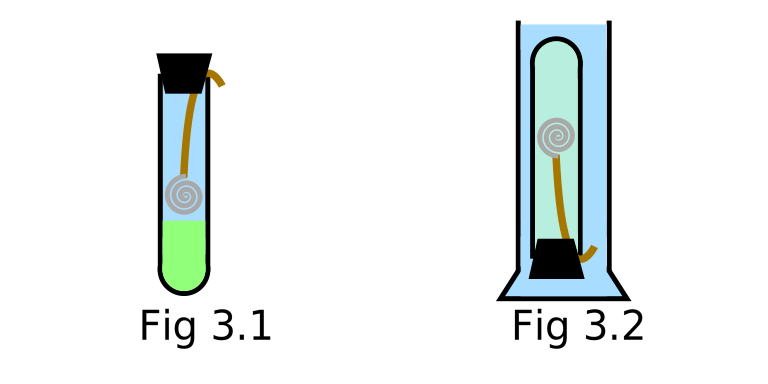
\includegraphics[width=\textwidth]{Apparatus}
Figure 3.1 shows the magnesium being held by the copper string, with the hydrochloric acid at the bottom of the gas collecting tube. Figure 3.2 shows the gas collection tube inverted, in the graduated cylinder, with the HCl distributed throughout the water. 
\subsection{Procedure}
\begin{enumerate}
	\item Fill the 2000 ml cylinder with tap water to the 2000 ml mark. Put the cylinder inside the large basin in order to contain any water spillage. 

	\item Obtain a piece of magnesium (Mg) ribbon from the instructor, and determine its mass. 
	\item Fold the ribbon length-wise into a tight square and wrap it in a cage of copper wire. The aim here is to try to \textit{encase} the magnesium ribbon completely with wire. The reason for this is so that the magnesium does not float away. 
	\item Obtain a 100 ml gas collection tube and, without splashing, fill it with approximately 15 ml of 6 M hydrochloric acid (HCl). Hydrochloric acid is the excess reactant in this reaction. Magnesium is the limiting reactant. 

	\item Fill the gas collection tube the remainder of the way with tap water \textit{slowly} until it is "full-to-the-brim.” There should not be any air bubbles when the tube is assembled.

	\item Hook the copper wire over the side of the tube with the magnesium in the water/acid mixture and carefully insert the rubber stopper into the water making sure it is sealed. The tube must be completely filled. Make sure that the copper wire is securely held by the stopper. 

	\item Cover the hole in the stopper with a finger, and invert the tube into the 2000 ml cylinder of water. The acid, being more dense than water, can be seen falling down through the water and it eventually reacts with the metal. Allow the reaction to go to completion. Do not let the magnesium strip fall through the hole in the stopper. All the hydrogen gas (H$_{2}$) must be collected in the gas collection tube. 
	 
	\item After the reaction stops, lower or raise the tube until the level of the liquid inside the tube is even with the level of the water outside the tube. This permits a measurement of the volume of the gases (hydrogen and water vapor) in the glass tube at room pressure. Record the room temperature, and use the chart provided to determine the pressure of water vapor at this temperature. Record the atmospheric pressure (room air pressure) placed on the board by the teacher. 
	 
	\item \textit{Read} and \textit{record} the volume of the gases in the tube. This must be done when the water levels are even inside and outside the tube. The reading yields the volume of the hydrogen gas. 
	 
	\item Carefully clean up the glassware by pouring the water and acid down the sink. Rinse the tube with tap water.
	
\end{enumerate}

\section{Data Table}
\begin{tabular}{ | l | l | l | l |}
\hline \textbf{\large{Substance}} & \textbf{\large{Property}} & \textbf{\large{Value}} & \textbf{\large{Unit}}\\ \hline
	Magnesium 	& Mass 			& 0.0780  & g\\ \hline
	Atmosphere 	& Pressure 		& 29.98 & inHg \\ \hline
	Water 		& Temperature 	& 22.0 	& $^\circ$C\\ \hline
	Water 		& Pressure 		& 19.8 	& mmHg\\ \hline
	Hydrogen 	& Volume 		& 78.15 & ml\\ \hline
\end{tabular}

\section{Observations}
	\subsection{Before Reaction}
	When outside the tube, the magnesium was silvery and shiny. When it was in the tube, was "floating" in the middle of the tube, and it was attached to a string of copper that held it in place. The magnesium was light silver in color, and bent into a small ball. The liquid that it was placed in was clear and colourless, and appeared to be stagnant.
	\subsection{During Reaction}
	The magnesium was bubbling rapidly, and a pocket of hydrogen gas was forming at the top of the tube. At first, the pocket grew very slowly, but eventually the rate of the reaction sped up, and the area directly next to the tube grew warmer by a very small amount.

\section{Analysis and Results}
\subsection{Theoretical Hydrogen Gas Amount}
The equation for the reaction is \\

Mg + 2HCl $\rightarrow$ MgCl$_{2}$ + H$_{2}$ 
\\ \\
We started off with 0.0780 grams of magnesium. Thus, we have \\

0.0780 \sout{grams Mg} $\times \frac{\textrm{1 mole Mg}}{\textrm{24.305 \sout{grams Mg}}}$ = \textbf{0.00321 moles of Mg}
\\ \\
For every mole of magnesium, there is one mole of hydrogen gas. This gives \\

0.00321 \sout{moles Mg} $\times \frac{\textrm{1 mole H$_{2}$}}{\textrm{1 \sout{mole Mg} }}$ = \textbf{0.00321 moles of H$_{2}$} 
\\
\subsection{Pressure of Hydrogen Gas}
We can use Dalton's Law of Partial Pressure to calculate the pressure of the hydrogen gas. Since the total pressure is equal to 29.98 inHg, we first convert the pressure value into mmHg to get \\

29.98 \sout{in}Hg $\times \frac{\textrm{25.4 mm}}{\textrm{1 \sout{in} }}$ = \textbf{761.5 mmHg} 
\\ \\
The temperature of the room at this time was 22$^\circ$C, and based on the data table given to us, the water pressure would be 17.5 mmHg. We now apply Dalton's Law of Partial Pressure to calculate the pressure of the hydrogen gas as \\

P$_{H_{2}}$ = P$_{total}$ - P$_{water}$ = 761.5 mmHg - 19.8 mmHg = \textbf{741.7 mmHg}
\\
\subsection{Actual Hydrogen Gas Amount}
We apply the Ideal Gas Law to determine the number of moles of hydrogen gas that was actually created. First, we convert the pressure of hydrogen gas into atmospheric pressure units (ATM) as \\

741.7 \sout{mmHg} $\times \frac{\textrm{1 ATM}}{\textrm{760 \sout{mmHg} } } = \textbf{\textrm{0.976 ATM}}$  \\
\\
Next, we convert 78.15 mL into L to get \\ 

78.15 \sout{mL} $\times \frac{\textrm{1 L}}{\textrm{1000 \sout{mL} } } = \textbf{\textrm{0.07815 L}}$  \\
\\
Then, we apply the data calculated so far to the Ideal Gas Rule to determine the number of moles of hydrogen gas formed using the following steps: \\

$P \times V = n \times R \times T$\\

$\textrm{or, 0.976 ATM} \times \textrm{0.07815 L} = \textrm{n moles} \times  \frac{\textrm{0.08205 joules}}{\textrm{mole} \times \textrm{Kelvin}} \times \textrm{295.15 Kelvin}$ \\

$\textrm{or, 0.07627 ATM} \times \textrm{L} = \textrm{n} \times \textrm{24.2171 joules}$ \\

$\textrm{or, n} = \frac{\textrm{0.07627 ATM} \times \textrm{L}}{\textrm{24.2171 joules}} = \textrm{\textbf{0.00315 moles}} $ 
\\ \\
The total amount of hydrogen gas that was actually formed is \textbf{0.00315 moles}. \\ The amount of hydrogen gas that should have been formed based upon the amount of magnesium used in the reaction is \textbf{0.00321 moles}. The discrepancy in these values comes from errors in the setup and execution of the experiment, as well as errors in measurement. We can use these two values to calculate the (negative) percent error for this  experiment as \\

$\textrm{100} \times \frac{\textrm{0.00315 moles - 0.00321 moles}}{\textrm{0.00321 moles}} = \textrm{\textbf{−1.87\%}}$ \\

\subsection{Results Table}
\begin{tabular}{ | l | l | l | l |}
\hline \textbf{\large{Substance}} & \textbf{\large{Property}} & \textbf{\large{Value}} & \textbf{\large{Unit}}\\ \hline
	Hydrogen Gas 	& Actual Amount 		& 0.00315 & moles\\ \hline
	Hydrogen Gas 	& Theoretical Amount 		& 0.00321 & moles\\ \hline
	Error 			& Percentage 				& -1.87\% 	& $^\circ$C\\ \hline
\end{tabular}
\\
\section{Conclusions and Error Analysis}

\subsection{Percent Error and Error Analysis}
The overall percent error for this experiment was \textbf{-1.87\%}, meaning that less hydrogen was actually produced compared to how much should have been produced.
During the setup of the experiment, there might have been air bubbles inside the tube when it was inverted to determine the volume of the hydrogen gas. This would be a positive error, because the gas whose volume would be measured would not be all hydrogen. While the copper basket was being constructed, and the magnesium string was being weighed, part of the string may have oxidized to form MgO. This would be an error in the negative direction, because there would be less overall hydrogen produced because the MgO would react to form water rather than hydrogen gas. Another source of error is in the reported atmospheric pressure. Since the pressure was not taken inside the room itself, it was not completely accurate. It cannot be determined whether this would be a positive or negative error due to the fact that the actualy pressure in the room at the time of experimentation was not measured. 

\subsection{Discussion Questions}
\begin{enumerate}
	\item \textit{Using chemical principles that you have learned this year, explain why you used copper wire to make the 
basket that held the magnesium in place instead of another material.} \\ \\ A basket was needed to hold the magnesium to prevent it from moving throughout the fluid, because that would cause problems with the consistency. Copper wire was a good choice for holding the magnesium in place because copper does not react with hydrochloric acid. Therefore, it was a good material for holding the magnesium in place without otherwise affecting the setup. \\
	\item  \textit{ Why did the magnesium not begin reacting immediately after you placed it into the tube? What action was 
required in order to start the reaction? } \\ \\ At first, the hydrochloric acid was completely at the bottom of the solution, because it is more dense than water, and thus would have sunk to the bottom, where it would not come into contact with the magnesium. In order to start the reaction, the magnesium had to be forced to make contact with the acid. This was achieved by the action of inverting the tube.\\ 
	\item \textit{Suppose the magnesium ribbon had been sitting in our storage room for a while and had oxidized slightly 
(that is, a small percentage of it had turned into MgO) before it was used in this lab. How would this affect 
your measured volume of hydrogen gas? Explain. As part of your explanation, write the reaction that would 
occur between the MgO and the HCl.}\\ \\ If the magnesium ribbon had been oxidized, there would not be as much hydrogen gas produced because the magnesium oxide (MgO) would react with the hydrochloric acid (HCl) to form water (MgO + 2HCl $\rightarrow$ MgCl$_{2}$ + H$_{2}$O) and thus there would be more water in the tube and less hydrogen because some of the hydrogen gas would be used up in the creation of the water molecules. \\ 

	\item \textit{In the reaction of magnesium with hydrochloric acid, how many total electrons are transferred? What 
species is oxidized, and what species is reduced?}\\ \\In the reaction between magnesium and hydrochloric acid, the magnesium loses two electrons, and transfers one to each of the hydrogen atoms, and thus two electrons are transformed. The hydrogen atoms do not lose any electrons, rather, they gain two (each gains one from magnesium), and then they create a covalent bond among themselves. Magnesium is oxidized because it loses electrons, and hydrogen is reduced because it gains electrons.              
\end{enumerate}
\subsection{Conclusions}
In this lab experiment, magnesium was made to react with hydrochloric acid to create pure hydrogen gas. The chemical equation for the reaction is

Mg + 2HCl $\rightarrow$ MgCl$_{2}$ + H$_{2}$ \\
The amount of hydrogen gas that should have been created from the 0.780 grams of magnesium used is \textbf{0.00321 moles}. The amount of hydrogen gas that was actually created in the reaction is \textbf{0.00315 moles}. The percent error in moles of hydrogen gas is \textbf{-1.87\%}. \\ \\ The purpose of this lab experiment was to try and demonstrate what happens when gas is produced in a chemical reaction inside a closed system. This lab experiment helps students understand the stoichiometry problems associated with the volume, temperature, mass, and pressure of gases.

\end{document}
